% test.tex
\title{Real Relevant Reviews ($R^3$): \\
Only The Most Helpful Product Reviews}

\author{Jen Darrouzet\cite{author1} and Bradley Nott\cite{author2}}

\newcommand{\abstractText}{\noindent
It gets harder each day for shoppers to wade through the ever-increasing number of online product reviews.  High-quality reviews that speak the language of the buyer can be tremendously helpful, but it is easy to become overwhelmed by a flood of meaningless, contrasting, untrustworthy and irrelevant opinions, leading to “analysis paralysis” that can derail a purchasing decision. The system that solves this problem would be popular with shoppers, and thus helpfulness prediction is an active area of research in both academia and industry. This paper investigates several predictive models and identifies several aspects found to be indicative of product review helpfulness. Building on one of these neural network models, we further propose a transfer learning method using BERT to rank helpful reviews that are most relevant to a shopper’s query. As we describe, these capabilities could be wrapped into a single “Real Relevant Reviews ($R^3$)” system that could support faster decision-making in  the online shopping process.
}

%%%%%%%%%%%%%%%%%
% Configuration %
%%%%%%%%%%%%%%%%%

\documentclass[10pt, a4paper, twocolumn]{article}
\usepackage{xurl}
\usepackage[super,comma,sort&compress]{natbib}
\usepackage{abstract}
\usepackage{lipsum}
\renewcommand{\abstractnamefont}{\normalfont\bfseries}
\renewcommand{\abstracttextfont}{\normalfont\small\itshape}
\usepackage{graphicx}

% Any configuration that should be done before the end of the preamble:
\usepackage{hyperref}
\hypersetup{colorlinks=true, urlcolor=blue, linkcolor=blue, citecolor=blue}
%%%%%%%%%%%%%%
% References %
%%%%%%%%%%%%%%

% If changing the name of the bib file, change \bibliography{test} at the bottom

\begin{document}

%%%%%%%%%%%%
% Abstract %
%%%%%%%%%%%%

\twocolumn[
  \begin{@twocolumnfalse}
    \maketitle
    \begin{abstract}
      \abstractText
      \newline
      \newline
    \end{abstract}
  \end{@twocolumnfalse}
]

%%%%%%%%%%%
% Article %
%%%%%%%%%%%

\section{Introduction}

Every day, online shoppers confront numerous opinions about products - reflected in $\star$ ratings, “best-seller” labels, and a seemingly endless supply of raw text reviews. On many websites, shoppers are commonly required to manually filter through text reviews using a combination of keyword tags and rating categories. This is a rather cumbersome search strategy, and we feel a guided approach is far more appropriate. We see an opportunity to create greater personalization in product recommendations through a more-efficient use of these text reviews. Ideally, to streamline the buying decision, websites should provide a personalized short list of reviews that are tuned to the interests of a particular shopper. However, even if a site maintains information on each shopper’s tastes, incentives might not be in alignment to provide the most helpful reviews to every shopper (e.g., ecommerce sites may prefer to display positive reviews in order to maximize sales revenues).

Therefore we envision a 3rd-party app, or browser plug-in, that could sift through reviews and display only the most helpful. Let’s call this hypothetical tool “RealRelevantReviews” ($R^3$). Functionally, a shopper could provide $R^3$ with a product-related query and receive a short collection of text reviews that contain both relevant and helpful content. To succeed, the system must be able to automatically determine whether or not a review contains helpful content. We propose that the reviews could each be categorized according to their helpfulness using a classification model trained with crowdsourced evaluations of product reviews.

If such a model is able to consistently classify unevaluated reviews, then $R^3$ might change the way shoppers interact with product reviews. Instead of conducting their own search through a collection of text reviews, shoppers could be quickly guided to an informed decision with the help of high-quality personalized content.



\section{Background}
Making sense of an ever-growing number of online product text reviews is an area of significant research. Common approaches focus on summarization techniques that attempt to condense collections of related reviews into a set of core concepts. In this context, individual text reviews are often thought to be a combination of product aspects and associated sentiments\cite{mcauley_2015}. Previous research has focused on methods to engineer or extract these types of features from text reviews in order to score and rank useful information\cite{hu_liu_2004}, \cite{bhure_pranav_2015}, or to generate structured extractive summaries\cite{kim2011comprehensive}.

Another popular approach to analyze text reviews is to identify and model the reviews that customers find helpful\cite{diaz_ng_2018}. Features that are often used to predict helpfulness include aspects of the reviews (e.g. length, sentiment, syntax, vocabulary, etc.) as well as attributes of the reviewer (e.g. experience, reputation, social network, etc.). These features support a variety of machine learning tasks such as predicting a helpfulness score using regression\cite{kim_2006}, or making a helpfulness classification decision\cite{malik_hussain_2017}.

This study is also aimed at the helpfulness classification problem. Specifically, we focus on whether or not a customer would consider a particular text review helpful, given a product of interest and a desired outcome with that product. While much of the previous research on this problem involves the careful use of feature engineering and metadata, we envision an approach that takes advantage of crowdsourced helpfulness votes to simplify the problem. If helpfulness votes consistently reflect the type of information that can enable a classification decision, then it might be possible to harness these relationships to train a model without additional feature engineering. Currently available product review datasets, such as the Amazon book reviews used in this work, along with a recent direction adjustment in research that favors neural networks and transfer learning are helping to advance the field in this direction\cite{diaz_ng_2018}. If our approach proves useful, it could then enable a service such as $R^3$ to efficiently serve customers a helpful and personalized subset of reviews, minus domain-specific feature engineering.

Noise complicates this challenge. Helpful reviews are rare events; review data is heavily imbalanced toward a class of reviews that are not helpful. The characteristics that determine helpfulness are also known to vary across product types\cite{diaz_ng_2018}. For example, text review features that are helpful to shoppers seeking consumer goods (e.g., a standardized test prep book) may be quite different from the features desired by those seeking experiences (e.g., a funny “beach read”).  Research also shows that reviews receive votes relative to the other reviews for the same product. Patterns such as this one, that reduce the average correlation between helpfulness votes and the content quality of an associated review, might result in an upper limit in the performance of a model trained in the manner that we suggest.

Nevertheless, we hope to show that crowdsourced helpfulness votes can be a reliable measure of the latent meaningful features contained in a text review. Additionally, we hope to shed light on the hidden components that determine how a review might be correctly classified as helpful. Our use of helpfulness votes as a source of signal is not entirely new. However, we believe that the manner in which we use helpfulness votes to support a classification task is a more meaningful use of this information than we have seen in related research.

\section{Data}

In this project, we constrain our scope to a dataset of 8 million book reviews published between May 1996 and July 2014 on Amazon.com (specifically the 5-core book set)\cite{mcauley_2015}. Fields available for each review include those listed in Table 1, and we make extensive use of the review text, the review's overall (1-5 $\star$) rating, the review date, and the review's earned helpful vote tally.  “asin” is the unique Amazon product ID, used for grouping by book (the review in Table 1 is from the book “The Other End of the Leash: Why We Do What We Do Around Dogs”). “helpful” is a tuple containing both the count of the review’s helpful votes, and the review’s unhelpful votes. (Amazon actually discontinued use of the “unhelpful” button after this dataset snapshot was saved.) “overall” is the count of $\star$s awarded the book by the reviewer. “reviewText” is the unstructured raw text provided by the reviewer, and “reviewTime” is the date the review was  published.
\\
\\
\begin{table}
\begin{tabular}{ | l | p{4cm}| }
  \hline
  Fieldname & Sample Value \\
  \hline
  asin & 034544678X \\
    \hline
  helpful & [3, 3] \\
    \hline
  overall & 5 \\
    \hline
  reviewText & I really enjoyed this book. It is a book on dog behavior, and provides only a few actual training tips. However, the author gives many... \\
    \hline
  reviewTime & Feb 20, 2005 \\
  \hline
\end{tabular}
\caption{Example book review record (our unit of analysis), see explanation in Data section.}
\end{table}

\begin{figure}[ht]
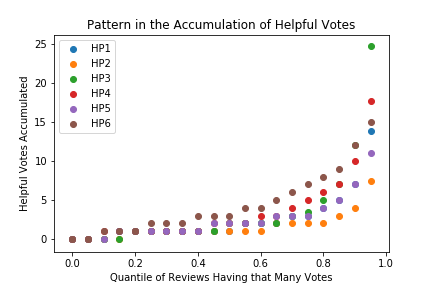
\includegraphics[width=3.25in]{HP_reviews_helpful_vote_accumulation.png}
\caption{Helpful vote tallies for reviews of six Harry Potter volumes published by mid 2013. }
\end{figure}


\begin{figure}[ht]
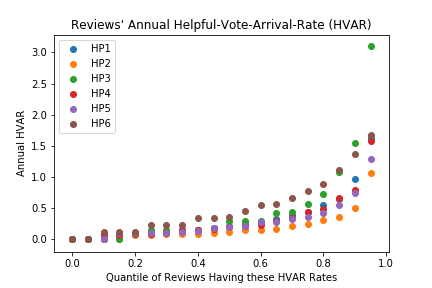
\includegraphics[width=3.25in]{HP_reviews_annual_HVAR.png}
\caption{Sample Annual HVAR metrics earned by reviews for the six Harry Potter volumes.}
\end{figure}

This investigation does not use all 8 million reviews from the dataset. We dropped about 4 million reviews that never received any helpful or unhelpful votes, as we could not guarantee such reviews had ever been shown for shoppers to vote upon. We also dropped reviews less than one year in age, as we chose to normalize the helpful vote counts to form a metric that we call the annual “helpful vote arrival rate” (HVAR, see side-by-side in Figure 1 and Figure 2). Further, we dropped books that had fewer than 4 reviews in our training set, and books without variance in their reviews’ HVAR metrics. Our dataset ultimately represents approximately 2.66 million reviews describing over 300,000 unique books.


It is important to point out that reviews for different products do not share similar opportunities to accumulate high HVAR values. For example, because BookA may be aimed at a wide audience, with plenty of marketing budget behind it, this book may receive multiple orders of magnitude more reviews than BookB (which could be a niche book about surviving with a rare disease, for instance). Fewer shoppers may consider purchase of BookB in this case, and so BookB’s reviews may receive very few votes of any kind. It would be unreasonable, then, to expect the HVAR metric to be directly comparable for ReviewA, written about BookA, and ReviewB, written about BookB, even if they were of equal quality. For this project, then, we isolated the quality signal by book (examining HVAR distributions grouped by “asin”).

Finally, in the introduction, we reflected that incentives for ecommerce sites prompt such vendors to display glowing (hyper-positive) reviews, in order to maximize sales. EDA reflects that critical reviews, however, can be most helpful to shoppers, see Figure 3. For example, our dataset’s review with the highest annual helpful-vote-arrival-rate (HVAR = 10264) is a 2$\star$ rating for "Fifty Shades of Grey". In order for our model to be able to learn helpfulness on both ends of the spectrum, and because 4-5$\star$ reviews make up nearly three-quarters (74.3\%) of our dataset, we stratified the dataset by overall $\star$ rating prior to conducting our random data splitting.

\begin{figure}[ht]
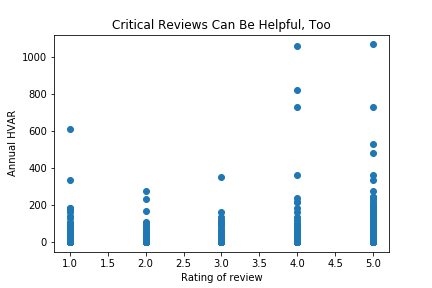
\includegraphics[width=3.25in]{Annual_HVAR_by_rating_37K_rsample.png}
\caption{Across a random sample of 37,722 reviews, shoppers can find both glowing and critical reviews helpful.}
\end{figure}

\section{Methods}
\textbf{Training a Review Classifier}
In order to frame the problem as a classification task we used the annual HVAR metric to facilitate grouping reviews into two classes. In its raw form the metric provides a meaningful way to compare reviews for the same product, but it is not directly useful for comparing reviews across products. This is because the metric values have a unique scale and distribution depending on the product. To solve this problem, we first grouped the data by product and standardized the HVAR values using Z-score normalization. The data was then ungrouped and these rescaled values were discretized into two integer class labels using a one-dimensional k-means clustering. We aimed to isolate and boost the "helpful" versus "definitely not helpful" signals. This procedure helped place high-signal reviews in the same class, regardless of the book that the review covers.

For this project’s classifiers, we chose to represent each review as a concatenation of its overall $\star$ rating with its raw text of maximum length 200 tokens. We did not use an integer or real number of $\star$s, but instead substituted categorical text according to the following mapping of $\star$s awarded to category text: {5$\star$s:’BEST’, 4$\star$s:’GOOD’, 3$\star$s:’OK’, 2$\star$s:‘BAD’, 1$\star$:‘WORST’}. We literally put words in the mouths of reviewers here (introducing bias), but in our judgement this was the most appropriate way to pass the overall $\star$ rating to the multiple models for an apples-to-apples comparison, for benchmarking purposes.

\textbf{Baseline for helpfulness prediction}
The most common class of online review is the unhelpful one. If the $R^3$ system guessed all reviews were unhelpful, it would be correct nearly three-quarters of the time, but be a useless system (it would never display any reviews to shoppers). As a more reasonable baseline instead, we trained a logistic regression model using tf-idf repersentations for text reviews and a subsample of the data with balanced classes.

\textbf{LSTM for helpfulness prediction}
Next we explored an LSTM model. We used Glove embeddings of 300 dimensions and trained a neural network model with a single bidirectional LSTM layer, with a binary output layer to make class predictions.

\textbf{BERT for the intersection of helpfulness and relevance}
We also tested BERT\cite{devlin2018bert}, to see how transfer learning would perform by comparison, mainly because we imagined that BERT's Next Sentence Prediction feature could add additional power to the $R^3$ system. For helpfulness classification and for NSP, we used 200 tokens maximum sequence length. For relevance, we treated the query as the second segment and the review as the first segment, having the BERT model output the probability that the content of the 2nd segment (the user query) is entailed in the 1st segment (the helpful book review).

While we did not pipeline the end-to-end system in this short period of time, it is our end goal to perform helpfulness classification offline (perhaps nightly for new reviews) storing a representation of each review such that - at shopper query time - the query could be run through a somewhat short-cutted NSP model, alongside a very short list of the most helpful reviews for that book. The shopper need only browse through a handful of reviews that had soared through all of $R^3$'s curation gates.

\section{Results}
\textbf{Classification of Helpfulness}
Results of the comparative helpfulness classification models are displayed in Table 2.

\begin{table}
\begin{tabular}{ | p{3cm} | p{3cm}| }
  \hline
  Tf.Idf-LR & Accuracy: 76.52\%, F1: 76.51\% \\
  \hline
  LSTM & Accuracy: 76.68\%, F1: 76.65\% \\
    \hline
  BERT & Accuracy: 74.31\%, F1: 74.27\% \\
  \hline
\end{tabular}
\caption{Comparison of review helpfulness classifiers. All were tested on a test split which was 50\% helpful and 50\% unhelpful. Future work to include unlabeled data with natural distributions.}
\end{table}

\noindent
\textbf{Addition of Relevance}
We prototyped using BERT’s NSP capability to find and rank reviews most applicable to the $R^3$ user’s query. Human inspection of the results look very promising, see Table 3.

\begin{table}[ht]
\begin{tabular}{ | p{7cm} | }
  \hline
  \textbf{Real Relevance}  \\
  \hline
  5$\star$: \textit{Jacob Jankowski recounts the wonderful time he spent with the Benzini Brothers Most Spectacular Show on Earth. During the Great Depression, his parents are killed and Jacob, now penniless, \textbf{has to leave vet school}...} \\
   \hline
  4$\star$: \textit{...Jacob's parents died just as he was about to write \textbf{his final exams in veterinary school} at Cornell University....because of his vet training, he ends up hired on to care for the horses and other animals...I read it quickly and found it very sweet and entertaining; \textbf{recommended for teens and adults}... Caveat: there are descriptions of mistreatment and abuse of animals in this book. If that is unpalatable to you, you should skip this book...} \\
   \hline
  2$\star$: \textit{Jacob, now an old man, begins the book by going back into his youth to the time \textbf{he was attending vet school}.  Tragic events turn his life upside down and he decides to run (literally).  He winds up with a circus and becomes the circus vet, although, he rarely spent any time with or working on the animals. He just stood and watched animals be slaughtered and then felt bad that he did not do anything...}\\
  \hline
\end{tabular}
\caption{Example reviews returned in top 10 most relevant to sample query:
 \textbf{“good for a teenager headed off to veterinary school?”}}
\end{table}

\section{Discussion}
Because review quality/helpfulness can be so subjective, we assembled a short list of reviews that we considered solidly helpful or unhelpful, and a few we found tripped up the systems again and again. We referred to these as our “canaries in the coal mine” set, and - in addition to accuracy scores like precision, recall, and f1 - we used these for comparative evaluation of the models’ errors.  Several of these example “canaries” are shown in Table 4, along with how long they accumulated votes, their total helpful vote counts and earned annual HVARs.


\begin{table*}[t]
  \centering
  \begin{tabular}{| p{8cm} | p{8cm} |}
      \hline
    \textbf{Well-Classified as Helpful - 5$\star$}  &
\textbf{Well-Classified as Helpful - 1$\star$} \\
\hline
    \textit{Noted historian of the early church Elaine Pagels has produced a clear, cogent, and very effective introduction to the subject of Gnosticism, a different form of Christianity that was declared heretical and virtually stamped out by the orthodox church by the start of the second century after Christ.  Most of what we knew of the Gnostic belief system came from the religious authors who worked so hard to destroy the movement…}  & \textit{Colin Campbell is so intent on promoting a vegan data that he misrepresents the data in the real China Study and cherry picks anti-animal food data.  For instance, he rightly cites the link between milk and autoimmune disease but fails to mention that gluten, from wheat and related grains, is at least as important a cause...  He makes completely false statements like folate not being in meat when organ meats are much higher in folate than any plant source according to the USDA.…} \\
    \hline
    Age: 11yrs   Helpful Votes: 788    Annual HVAR: 74.4
& Age: 5yrs      Helpful Votes: 332  Annual HVAR: 69.01
\\
\hline
    \textbf{Well-Classified as Unhelpful: 5$\star$}  & \textbf{Well-Classified as Unhelpful: 1$\star$} \\
    \hline
    \textit{Just downloaded this series.  Looking forward to getting to read it, once i get past some of the other books on my reading list.  I just love beig able to carryall these books without having to carry them individually!} & \textit{I like to read many different books from many points of view.  This book was a complete waste of time that I will never get back. Save yourself the trouble and money.} \\
    \hline
    Age: 2yrs   Helpful Votes: 0     Annual HVAR: 0 & Age: 3yrs   Helpful Votes: 51   Annual HVAR: 18.84\\
    \hline
  \end{tabular}
  \caption{Examples of classification results that meet expectations}
  \label{tab:1}
\end{table*}

In Table 5 we see an example of a problematic review. The model classified this long and detailed review as probably helpful, when it is not really helpful at all (it received zero votes from Amazon shoppers, likely because it isn’t really a book review; it is instead a review of shipping fulfillment performance). We found several examples of such “fulfillment” reviews and looked into how they were, or were not, tripping up the algorithm. We chose to employ LIME\cite{Ribeiro_2016} - which allows model-agnostic decision introspection - to learn more about how BERT was making its choices. Figure 4 reveals what we can blame for the misclassification of the 1$\star$ video game guide review; note contrasting Figures 4 and 5, both handling fulfillment reviews.

\begin{table}
  \begin{tabular}{| p{7cm} |}
      \hline
\textbf{Misclassified as Helpful - 1$\star$} \\
\hline
 \textit{Im giving this one star for now. i think i can update it later can I?I just want to say right now if you really want this guide you might be better of finding it in a store. this is the 2nd time in 6 months that amazon has screwed up a video game guide order i had.I ordred this guide at 5:30 pm est yesterday when it said i still had time to order it to get it by today.. then they tell me the order was delayed and i wont get it till Monday.WHY? The item lists on the page right now that its avalible for saturday delivery yet they refused to make sure the package would get to me then.I cant cancel it and order another one in hopes it will get here saturday because "its in processing"Very frustrated. very poor handling by amazon. yeah they refunded the amazon prime one day shipping fee. but they still could have updated it to saturday delivery!…} \\
    \hline
Age:2yrs     Helpful Votes: 0    Annual HVAR: 0
\\
    \hline
  \end{tabular}
  \caption{The above example highlights a shortcoming of the classifier, see text for explanation.}
\end{table}

\begin{figure}[ht]
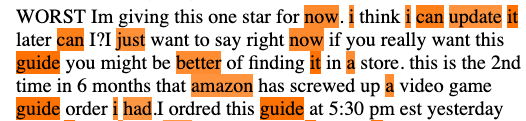
\includegraphics[width=3in]{LIME_review_of_shipping_video_game_guide.png}
\caption{Misclassified 1$\star$ review from Table 5 has highly-weighted word “guide” - which the model must have learned is a generally helpful concept.}
\end{figure}

\begin{figure}[ht]
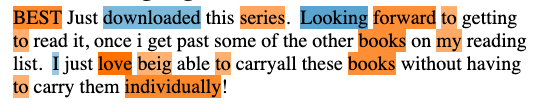
\includegraphics[width=3.25in]{LIME_review_just_downloaded.png}
\caption{Well-classified 5$\star$ review is recognized as unhelpful, primarily due to the word “downloaded” - likely an indicator of the fulfillment topic.}
\end{figure}

One fairly common word - "claim(s)" - seemed to indicate review helpfulness with some reliability. Approximately 3.3\% of reviews have this string, and conditional on its presence, the review gathers an HVAR metric putting it in the helpful class 82.42\% of the time. This string did not always make it into the most important features in a LIME evaluation, but when it was in the list, it was unfailingly weighted on the side of helpfulness, as shown in Figure 6.

\begin{figure}[ht]
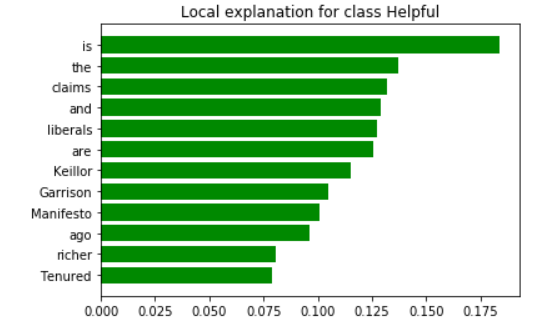
\includegraphics[width=3.25in]{LIME_claims_as_helpfulness_indicator.png}
\caption{1$\star$ review discusses a claim and is recognized as helpful by the model.}
\end{figure}

We initially thought this could be due to the detection of structured argumentation\cite{Lippi2016292} around nonfiction books, but we found the terminology in reviews of fictional works as well. The helpful review in Figure 7 describes a fictional character making a claim in a spy novel. Using the word "claim" perhaps indicates the difference between believing things at face value and reserving judgment - something humans may value as especially helpful.

\begin{figure}[ht]
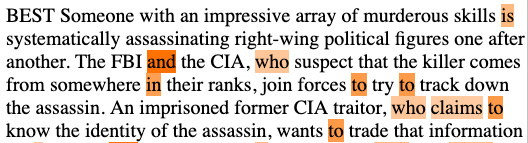
\includegraphics[width=3in]{LIME_fictional_review_character_claim.png}
\caption{Reviews that discuss a claim are highly likely to be determined helpful.}
\end{figure}


\section{Conclusion}
This study investigated methods for providing online shoppers with a short list of product reviews, scored using crowd-sourced helpfulness votes, that could efficiently and effectively inform shoppers’ individual buying decisions. From a dataset of millions of book reviews and associated helpfulness votes, we derived a simple metric, the annual helpful vote arrival rate (HVAR), for each review greater than one year in age.  We used this HVAR metric to label all reviews for books with sufficient review coverage and variance, and then developed three different types of models that could reasonably classify book reviews as either helpful or not.

A variety of techniques helped us identify several intriguing characteristics indicative of helpful reviews. None of the models had remarkable accuracy, likely due to the noisy data source (which included significant evidence of disagreement among humans, and some evidence of the review system being gamed).  We benchmarked the three models’ performance, and conducted error analysis.

Further, we proposed future work pursuing a promising extension of the BERT-based model. The BERT-based model has the capability to deliver truly individualized relevance in terms of the reviews delivered to a shopper. This extension relies on the Next Sentence Prediction features of the model, which - as shown - can incorporate a shopper’s specific query and return ranked results. This is our recommended approach for further development of the Real Relevant Reviews ($R^3$) system, which promises to deliver honest (both negative and positive) product reviews that are both remarkably helpful and remarkably relevant.

\nocite {yoon_2014,tf_movie_demo,lee_2019,nainan_2019}
\bibliography{foo}
\bibliographystyle{plain}
\begin{thebibliography}{1}

\bibitem{author1} Jen  Darrouzet {\em jend@ischool.berkeley.edu}

\bibitem{author2} Bradley Nott {\em bradley.nott@ischool.berkeley.edu}

\bibitem{hu_liu_2004} [M. Hu \& B. Liu, 2004] {\em Mining and Summarizing Customer Reviews} Proceedings of ACM SIGKDD

\bibitem{kim_2006} [Soo-Min Kim et al, 2006] {\em Automatically Assessing Review Helpfulness} Proceedings of the 2006 Conference on Empirical Methods in Natural Language Processing

\bibitem{kim2011comprehensive} [Hyun Duk Kim et al, 2011] {\em Comprehensive review of opinion summarization}

\bibitem{yoon_2014} [K. Yoon, 2014] {\em Convolutional Neural Networks for Sentence Classification} Proceedings of the 2014 Conference on Empirical Methods in Natural Language Processing

\bibitem{bhure_pranav_2015} [Bhure \& Pranav, 2015] {\em BOOK RECOMMENDATION SYSTEM USING OPINION MINING TECHNIQUE} International Journal of Research in Engineering and Technology

\bibitem{mcauley_2015} [McAuley et al, 2015] {\em Learning Attitudes and Attributes from Multi-Aspect Reviews} SIGIR \url{http://jmcauley.ucsd.edu/data/amazon/}

\bibitem{Lippi2016292} [Lippi \& Torroni, 2016] {\em "MARGOT: A web server for argumentation mining"} Expert Systems with Applications

\bibitem{Ribeiro_2016} [Ribeiro et al., 2016] {\em "Why Should {I} Trust You?" - Explaining the Predictions of Any Classifier} Proceedings of the 22nd {ACM} {SIGKDD} International Conference on Knowledge Discovery and Data Mining

\bibitem{malik_hussain_2017}[Malik \& Hussain, 2017] {\em Helpfulness of product reviews as a function of discrete positive and negative emotions} Computers in Human Behavior

\bibitem{diaz_ng_2018} [Diaz \& Ng, 2018] {\em Modeling and Prediction of Online Product Review Helpfulness: A Survey} Proceedings of the 56th Annual Meeting of the Association for Computational Linguistics

\bibitem{devlin2018bert} [Devlin et al, 2018] {\em BERT: Pre-training of Deep Bidirectional Transformers for Language Understanding} arXiv preprint arXiv:1810.04805

\bibitem{tf_movie_demo} [Google, 2019] {\em Predicting Movie Review Sentiment with BERT on TF Hub} \url{https://colab.research.google.com/github/google-research/bert/blob/master/predicting_movie_reviews_with_bert_on_tf_hub.ipynb}

\bibitem{lee_2019} [Ceshine Lee, 2019] {\em News Topic Similarity Measure using Pretrained BERT Model} \url{https://medium.com/the-artificial-impostor/news-topic-similarity-measure-using-pretrained-bert-model-1dbfe6a66f1d}

\bibitem{nainan_2019} [Charles Nainan, 2019] {\em scikit-learn wrapper to finetune BERT} \url{https://github.com/charles9n/bert-sklearn}

\end{thebibliography}

\end{document}

% Create PDF on Linux:
% FILE=test; pkill -9 -f ${FILE} &>/dev/null; rm -f ${FILE}*aux ${FILE}*bbl ${FILE}*bib ${FILE}*blg ${FILE}*log ${FILE}*out ${FILE}*pdf &>/dev/null; pdflatex -halt-on-error ${FILE}; bibtex ${FILE} && pdflatex ${FILE} && pdflatex ${FILE} && (xdg-open ${FILE}.pdf &)
